% Estilo compartido. Compilar el volumen principal con XeLaTeX o Tectonic.
\documentclass[12pt,letterpaper]{article}
\usepackage[spanish,es-noshorthands]{babel}
\usepackage[left=23mm,right=23mm,top=23mm,bottom=22mm,headheight=15pt]{geometry}
\usepackage{graphicx,xcolor,fancyhdr}
\usepackage[unicode,pdflang={es-MX},bookmarksopen,colorlinks=true,linkcolor=azul]{hyperref}
% La familia Latin Modern de 10 puntos también cubre los títulos grandes.
\DeclareFontShape{TU}{lmr}{m}{n}{<->\UnicodeFontFile{lmroman10-regular}{\UnicodeFontTeXLigatures}}{}
\DeclareFontShape{TU}{lmr}{b}{n}{<->\UnicodeFontFile{lmroman10-bold}{\UnicodeFontTeXLigatures}}{}
\DeclareFontShape{TU}{lmr}{bx}{n}{<->\UnicodeFontFile{lmroman10-bold}{\UnicodeFontTeXLigatures}}{}
\DeclareFontFamily{TU}{lmtt}{}
\DeclareFontShape{TU}{lmtt}{m}{n}{<->\UnicodeFontFile{lmmono10-regular}{}}{}
\definecolor{azul}{HTML}{075479}
\definecolor{tinta}{HTML}{172F3D}
\definecolor{muted}{HTML}{455E6A}
\definecolor{niebla}{HTML}{EDF4F6}
\renewcommand{\headrulewidth}{0pt}
\setlength{\parindent}{0pt}
\setlength{\parskip}{4pt}
\setlength{\emergencystretch}{1.3em}
\linespread{1.08}
\pagestyle{fancy}\fancyhf{}
\fancyhead[L]{\small\color{muted}ESCOM \enspace / \enspace Trabajo Terminal 2026-B155}
\fancyhead[R]{\small\color{muted}\volumen}
\fancyfoot[L]{\small\hyperlink{indice}{Volver al índice}}
\fancyfoot[R]{\small\color{muted}\thepage}
\newcommand{\boton}[1]{\textbf{#1}}
\newcommand{\tema}[1]{\par\addvspace{9pt}{\large\bfseries\color{azul}#1\par}\nobreak}
\newcommand{\pagina}[3]{\clearpage\phantomsection\addcontentsline{toc}{section}{#2}%
{\small\bfseries\color{azul}\MakeUppercase{#1}\par}\vspace{2pt}%
{\raggedright\fontsize{23}{26}\selectfont\bfseries\color{tinta}#2\par}\nobreak\vspace{2pt}%
{\large\color{muted}#3\par}\vspace{4pt}}
\newenvironment{pasos}{\begin{enumerate}\setlength{\itemsep}{3pt}\setlength{\topsep}{1pt}\setlength{\parskip}{0pt}}{\end{enumerate}}
\newcommand{\nota}[2]{\par\addvspace{7pt}\noindent\begingroup\setlength{\fboxsep}{8pt}%
\colorbox{niebla}{\parbox{\dimexpr\linewidth-2\fboxsep\relax}{\small\color{tinta}\textbf{#1}\enspace #2}}\endgroup\par}
\newcommand{\captura}[4][1]{\par\addvspace{6pt}\begin{center}\setlength{\fboxsep}{0pt}%
\fcolorbox{niebla}{white}{\includegraphics[width=\dimexpr#1\linewidth-2\fboxrule\relax,height=#3,keepaspectratio]{figuras/#2.png}}%
\par\vspace{2pt}{\small\color{muted}#4\par}\end{center}}
\newcommand{\portada}[2]{%
\hypersetup{pdftitle={Manual de usuario. #1},pdfauthor={Díaz Ramírez Daniel y Téllez De La Cruz Esaul},pdfsubject={Aplicación web para la gestión de actividades de la ESCOM. TT 2026-B155}}
\color{tinta}\thispagestyle{empty}
\begin{minipage}[c]{.18\linewidth}
\includegraphics[width=.83\linewidth]{figuras/escudo-escom.png}\end{minipage}\hfill
\begin{minipage}[c]{.79\linewidth}{\large\bfseries Instituto Politécnico Nacional\par}Escuela Superior de Cómputo\par Trabajo Terminal 2026-B155\end{minipage}
\par\vspace{14mm}{\color{azul}\bfseries MANUAL DE USUARIO\par}\vspace{1mm}
{\fontsize{32}{35}\selectfont\bfseries #1\par}\vspace{2mm}
{\large Aplicación web para la gestión de actividades de la ESCOM\par}\vspace{4mm}
#2\par\vspace{4mm}
\hypertarget{indice}{}\tableofcontents
\vfill
{\small\color{muted}\textbf{Autores}\quad Díaz Ramírez Daniel y Téllez De La Cruz Esaul\par
\textbf{Directora}\quad Dra. Mónica Rivera De La Rosa\par
Edición de noviembre de 2026 \enspace · \enspace Ciudad de México\par}}
\AtBeginDocument{\renewcommand{\contentsname}{Índice de tareas}}

\newcommand{\volumen}{Comunidad escolar}
\begin{document}
\portada{Comunidad escolar}{Para visitantes, estudiantes y docentes. Consulta información del plantel, participa en un club, localiza a un profesor o coordina la devolución de un objeto. Elige en el índice la tarea que quieres realizar.}

\pagina{Acceso}{Crear una cuenta y recuperar el acceso}{Necesitas un navegador con conexión a internet y acceso a tu correo institucional. Para consultar contenido público basta con abrir la dirección de la plataforma que te proporcione la ESCOM.}
\begin{minipage}[t]{.52\linewidth}
\tema{Registrarte por primera vez}
\begin{pasos}
\item Abre \boton{Crear cuenta}. Escribe tu nombre y correo. Usa \texttt{@alumno.ipn.mx} si eres estudiante o \texttt{@ipn.mx} si eres docente.
\item Elige una contraseña de 8 a 72 caracteres. Puedes agregar la boleta o el número de empleado después, desde tu perfil.
\item Lee y acepta el aviso de privacidad. Pulsa \boton{Crear cuenta} y abre el mensaje de confirmación en tu buzón institucional.
\item Sigue el enlace y, si aparece, pulsa \boton{Confirmar y activar cuenta}. En \boton{Entrar}, escribe el correo y la contraseña. Tu inicial en la cabecera indica que iniciaste sesión.
\end{pasos}
\end{minipage}\hfill
\begin{minipage}[t]{.43\linewidth}\vspace{7pt}\centering
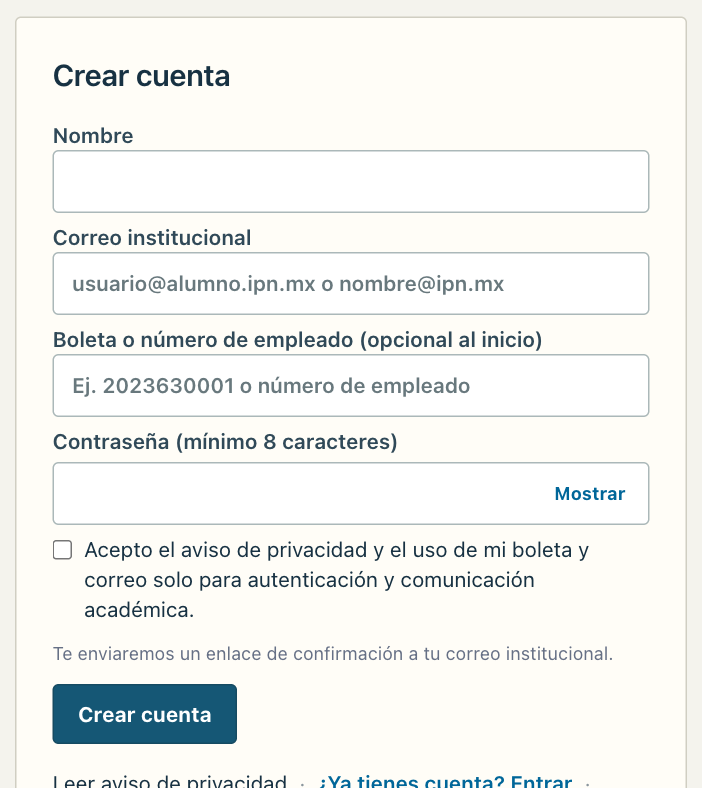
\includegraphics[width=\linewidth]{figuras/registro.png}\par{\small\color{muted}Formulario de registro institucional.}\end{minipage}
\tema{Recuperar tu contraseña}
En \boton{Entrar}, selecciona \boton{Olvidé mi contraseña}, escribe tu correo y pulsa \boton{Enviar enlace}. Abre el mensaje más reciente, continúa a la nueva contraseña, escríbela dos veces y pulsa \boton{Guardar contraseña}. Vuelve a entrar con ella.
\nota{Si no llega el mensaje}{Comprueba el dominio y la carpeta de correo no deseado. Si el registro sigue pendiente, usa el reenvío de confirmación. Para un enlace de recuperación vencido, inicia una nueva solicitud desde \textbf{Olvidé mi contraseña}.}

\pagina{Consulta pública}{Encontrar un aviso o un evento}{Desde Inicio puedes abrir publicaciones recientes. Para buscar una convocatoria usa Avisos. Para comprobar un horario o una sede usa Eventos.}
\captura{avisos}{53mm}{En Comunicados, los filtros de categoría y área se pueden combinar con una búsqueda.}
\tema{Encontrar y abrir un comunicado}
\begin{pasos}
\item En \boton{Avisos}, escribe una palabra del titular, por ejemplo «semestre». Elige una categoría y, si conoces la oficina emisora, selecciónala en el filtro de área.
\item Abre la tarjeta para leer el texto completo. Revisa la fecha y el área emisora. Si incluye un cartel, amplíalo. Si incluye un enlace oficial, ábrelo para consultar la convocatoria de origen.
\item Si faltan resultados, vuelve a \boton{Todos} y \boton{Todas las áreas}, quita el filtro de cartel y prueba una palabra más corta.
\end{pasos}
\tema{Consultar la cartelera y marcar asistencia}
En \boton{Eventos}, cambia de mes con las flechas del calendario o usa \boton{Próximos 7 días}. Selecciona un día o una sede y lee la fecha, la hora y la ubicación de la actividad. Si la selección está vacía, vuelve a todos los espacios o cambia de mes.
\par Con la sesión iniciada, pulsa \boton{Asistiré} en la ficha. La marca y el contador reflejan tu elección. Pulsa de nuevo para retirarla. La cartelera informa sobre actividades ya autorizadas por el plantel.

\pagina{Orientación escolar}{Seguir una guía y preguntar en el foro}{Usa una guía para preparar un trámite y el foro para aclarar una duda con la comunidad o el área responsable. La entrega de documentos sigue el procedimiento de la ventanilla correspondiente.}
\captura{foro}{55mm}{En Foro y Guías, selecciona Guías, Con respuesta oficial o Abiertas para acotar los resultados.}
\tema{Consultar un paso}
\begin{pasos}
\item En \boton{Foro y Guías} (en el móvil, \boton{Foro}), escribe el nombre del trámite y elige el área. Abre la guía que corresponda.
\item Elige \boton{Diagrama visual} para ver las rutas o \boton{Recorrido guiado} para avanzar paso a paso. En una decisión, selecciona la opción que describe tu situación. Consulta las preguntas frecuentes y descarga el formato PDF si aparece.
\item Para aclarar un requisito, abre ese paso y entra al mini-foro con tu cuenta. Envía la pregunta o sugiere la corrección concreta. Así el área puede identificar el paso afectado. El avance marcado en el catálogo se guarda en ese navegador.
\end{pasos}
\tema{Publicar una duda sin duplicarla}
Si la búsqueda no resuelve tu duda, pulsa \boton{Nueva publicación}. Con tu sesión iniciada, elige el área y el tipo, escribe un título y revisa las publicaciones parecidas. Abre una existente si ya cubre el tema. En otro caso completa los detalles y publica. En el hilo podrás leer las respuestas, votar su utilidad y reconocer la identificada como oficial. Si aparece un tiempo de espera, vuelve a intentarlo al concluir el plazo indicado.

\pagina{Clubes estudiantiles}{Solicitar ingreso o proponer un club}{La ficha de un club activo reúne los requisitos, los horarios y los medios de contacto. La pestaña Propuestas contiene las iniciativas que aún buscan respaldo o tramitan su registro.}
\captura{clubes}{59mm}{El directorio distingue clubes activos y propuestas. Los filtros permiten elegir el tipo de actividad.}
\tema{Ingresar a un club activo}
\begin{pasos}
\item Entra con cuenta de alumno. Abre \boton{Clubes}, busca el nombre o filtra por \boton{Académico}, \boton{Cultural} o \boton{Deportivo}. Selecciona \boton{Ver club}.
\item En \boton{Acerca y contacto}, consulta el horario y los requisitos. Pulsa \boton{Solicitar ingreso}. Si el club usa preguntas de admisión, respóndelas y envía la solicitud.
\item Mientras aparezca \boton{Solicitud pendiente}, espera la revisión del club. Regresa a la ficha o consulta la campana. Cuando se acepte tu ingreso podrás leer las publicaciones internas.
\end{pasos}
\tema{Respaldar o iniciar una propuesta}
En \boton{Clubes}, abre \boton{Propuestas}, selecciona la iniciativa y pulsa \boton{Me interesa} con tu cuenta de alumno. Verás el respaldo en el contador. Para crear una iniciativa, elige \boton{Nuevo club}, escribe nombre, tipo y objetivo, y revisa las coincidencias antes de enviarla. Abre la propuesta creada para dar seguimiento al expediente.
\nota{Dos acciones distintas}{El respaldo cuenta para formar un nuevo club. Si quieres ingresar a uno que ya opera, envía la solicitud desde la ficha de ese club.}

\pagina{Trámite de clubes}{Completar el expediente del club}{Abre el detalle desde Clubes, en Propuestas. Ahí aparecen la meta de respaldo, el avance documental, la coordinación docente y la cita. Cada participante aporta su parte desde su propia cuenta.}
\tema{1. Cada estudiante completa su expediente}
Al alcanzar la meta indicada en la ficha (20 respaldos por defecto), el proponente y los estudiantes que respaldaron capturan carrera y teléfono en \boton{Tu expediente individual}. Pulsa \boton{Guardar datos}. Selecciona un tipo de documento y carga el archivo correspondiente. Repite el proceso para credencial IPN, boleta o tira de materias, firma y vigencia de derechos IMSS. Se admiten PDF, JPG o PNG de hasta 10 MB por archivo. Comprueba el estado de los cuatro documentos. Si uno indica \boton{Corregir}, lee la observación y sustituye ese archivo.
\tema{2. El docente confirma la coordinación}
El alumno responsable busca e invita al profesor con su cuenta institucional. El profesor abre la propuesta con su propia sesión y acepta la coordinación. Si utilizan la opción por código, el docente comparte con el responsable el código de seis caracteres para validarlo en esa propuesta. Comprueba que el nombre aparezca como coordinador confirmado.
\tema{3. El responsable envía el registro formal}
Cuando la ficha habilite el formulario, el responsable completa el cronograma anual, las actividades, los espacios y horarios y la contribución a la comunidad. Indica el semestre y confirma la condición de alumno regular de tercero a séptimo semestre para presidir el club. Agrega las preferencias de cita si las tiene y envía el registro formal al área indicada.
\tema{4. Alumno y docente acuerdan la junta}
Cuando la oficina proponga horarios, ambos entran por separado y marcan su disponibilidad. Regresen a la ficha para consultar la fecha definitiva, modalidad y lugar o enlace. Atiendan las observaciones documentales y la revisión institucional. Tras el alta, el expediente muestra \boton{Ver el club registrado}.
\nota{Si el registro sigue bloqueado}{Revisa la meta de respaldos, los datos y documentos pendientes de cada estudiante y la confirmación del profesor. Haber alcanzado la meta abre la etapa documental.}

\pagina{Objetos perdidos}{Reportar una pérdida o un hallazgo}{Consulta primero los reportes abiertos. La ubicación y un rasgo visible permiten reconocer posibles coincidencias sin revelar el dato que solo conoce el dueño.}
\captura{objetos}{59mm}{En Objetos, los avisos de pérdida y los de hallazgo aparecen con etiquetas diferentes.}
\tema{Publicar un reporte}
\begin{pasos}
\item En \boton{Objetos}, usa \boton{Perdidos} o \boton{Encontrados} y revisa las fichas. Si ya existe una coincidencia, ábrela y continúa con la tarea de la página siguiente.
\item Con sesión iniciada, elige \boton{+ Reportar objeto} y selecciona \boton{Perdí algo} o \boton{Encontré algo}. Escribe título, descripción y lugar. Puedes adjuntar hasta dos fotos.
\item Para un hallazgo, escribe una pregunta llave y una respuesta esperada. Por ejemplo, si el objeto lleva una calcomanía en el interior, pregunta qué figura tiene. Reserva la figura y su respuesta para la validación privada.
\item Pulsa \boton{Publicar reporte}. Abre la ficha y revisa \boton{Posibles coincidencias} cuando aparezca. Compara descripción y lugar antes de contactar a la otra persona.
\end{pasos}
\nota{Si ya resolviste la pérdida por otro medio}{Abre tu reporte y selecciona \textbf{Cerrar reporte}. Para dejar constancia de una entrega acordada en la plataforma, usa el código de entrega que se describe en la página siguiente.}

\pagina{Objetos perdidos}{Reclamar y confirmar la entrega}{Intervienen dos personas. Quien publicó el reporte revisa la solicitud. Durante la devolución, el dueño muestra el código y quien tiene el objeto lo valida.}
\captura[.78]{pregunta-llave}{47mm}{La persona que encuentra el objeto configura la pregunta y conserva la respuesta de referencia.}
\tema{Abrir una solicitud}
Si ves tu pertenencia en un reporte \boton{Encontrado}, abre \boton{Reclamar este objeto}, responde la pregunta llave y envía. Si ayuda a identificarla, agrega detalles o un comprobante privado en JPG, PNG, WEBP o PDF de menos de 10 MB. Si tú encontraste algo que alguien reportó como \boton{Perdido}, usa \boton{¿Lo encontraste?} e indica dónde lo resguardas.
\tema{Revisar y coordinar}
Quien publicó abre su reporte, lee el mensaje y revisa el comprobante si lo hay. Aprueba la solicitud que corresponda o recházala si los detalles no coinciden. Una vez aprobada, ambas partes consultan \boton{Coordinación de entrega}, acuerdan un lugar y horario en ESCOM y pulsan \boton{Guardar nota de encuentro}.
\tema{Registrar la devolución}
\begin{pasos}
\item En el encuentro, el dueño abre el \boton{Código QR temporal de entrega} en su ficha.
\item Quien resguarda el objeto abre \boton{Confirmar entrega presencial}. Al entregarlo, escanea el QR, sube su captura o escribe los 12 caracteres. Confirma la operación.
\item Comprueben que el reporte figure como \boton{Entregado}. Si el código expiró, usen \boton{Renovar código QR (+24h)} y validen el nuevo. Si falla la cámara, usen la entrada manual.
\end{pasos}

\pagina{Mapa y directorio}{Localizar un espacio o a un profesor}{Usa el mapa para identificar el edificio y la planta. En el directorio puedes distinguir una ubicación confirmada de otra que la comunidad ha sugerido.}
\captura{mapa}{64mm}{Mapa del campus. El selector de planta y la pestaña del directorio ofrecen dos formas de buscar.}
\tema{Encontrar un espacio}
En \boton{Mapa}, usa la búsqueda de espacio o profesor. Selecciona el resultado para abrir su ficha. En \boton{Mapa interactivo 3D}, elige \boton{Planta baja}, \boton{Piso 1} o \boton{Piso 2} para ver el nivel correspondiente. Arrastra la vista o usa los controles de zoom. Vuelve a \boton{Todo 3D} para situar el edificio en el conjunto.
\tema{Encontrar o sugerir un cubículo}
Abre \boton{Directorio de profesores}, busca por nombre y consulta el código del cubículo o salón. Si el docente aparece en \boton{Sin cubículo} y conoces su ubicación, entra con tu cuenta, pulsa \boton{Sugerir cubículo}, elige el espacio y envía la sugerencia. Comprueba en la ficha si figura como propuesta o confirmada.
\tema{Registrar tu ubicación como docente}
Con tu cuenta de profesor, pulsa \boton{Colocar mi cubículo} o \boton{Mi cubículo} si ya tienes uno. Selecciona el código del espacio, revisa edificio y piso, escribe una etiqueta o referencia y guarda. Busca después tu nombre en el directorio para comprobar el cambio.

\pagina{Cuenta y seguimiento}{Revisar notificaciones y datos personales}{La campana reúne avisos dirigidos a tu cuenta. Tu inicial o nombre, en la cabecera, abre el perfil.}
\tema{Consultar y ajustar los avisos}
Abre la campana y selecciona \boton{Ver} para ir al elemento relacionado. También puedes marcar una notificación como leída o usar \boton{Marcar todas como leídas}. En las preferencias, elige los temas que deseas recibir dentro de la plataforma, por ejemplo clubes, foro u objetos, y pulsa \boton{Guardar preferencias}.
\tema{Corregir o descargar tus datos}
\begin{pasos}
\item Abre tu perfil. En \boton{Editar mi perfil} actualiza el nombre o la boleta o número de empleado y pulsa \boton{Guardar perfil}. En la misma pantalla puedes consultar tus insignias.
\item Para obtener una copia, abre \boton{Derechos ARCO y Privacidad} y elige \boton{Descargar mis datos (CSV)} para abrirlos en una hoja de cálculo o \boton{Descargar mis datos (JSON)} para obtener el archivo estructurado.
\item Para pedir rectificación, cancelación u oposición, o reportar un incidente, elige el tipo de solicitud, describe el dato y la acción que solicitas y pulsa \boton{Enviar solicitud ARCO / incidente}. Consulta la respuesta en \boton{Mis solicitudes registradas}.
\end{pasos}
\nota{Baja definitiva}{\textbf{Eliminar mi cuenta (Cancelación directa)} inicia la eliminación de la cuenta. Descarga antes los datos que quieras conservar. Para solicitar revisión previa, usa el formulario de derechos ARCO.}
\tema{Consultar una suspensión}
En \boton{Entrar}, abre \boton{Consultar o apelar una suspensión}. La consulta requiere identificarte con la cuenta afectada. Si puedes abrir la suspensión, lee el motivo, explica en al menos 20 caracteres qué solicitas revisar y pulsa \boton{Enviar apelación}. En esa ficha aparecen el estado y la respuesta. Si la pantalla vuelve a pedirte acceso, solicita ayuda a la administración de la plataforma con la fecha y el mensaje que viste.
\par Al finalizar en un equipo compartido, pulsa \boton{Salir} en la cabecera.
\end{document}
